\chapter{Tái hiện trò chơi Griductive}
\label{chap:game}

\section{Giới thiệu}
Nhóm xây dựng phiên bản Griductive bằng Python và Pygame, tham khảo luật chơi gốc~\cite{griductive,pygameDocs}. Trò chơi hỗ trợ bàn cờ $3\times3$, $4\times4$ và $5\times5$. Mỗi nhân vật có trạng thái ẩn là tội phạm hoặc vô tội; người chơi chỉ được mở thẻ khi kết luận được chứng minh từ thông tin công khai.

\section{Giao diện và các tính năng chính}
Giao diện gồm bàn cờ ở bên trái và bảng manh mối ở bên phải. Mỗi thẻ hiển thị tọa độ, tên, xuất xứ và ảnh nhân vật. Thẻ đã mở hiển thị thêm trạng thái cùng manh mối; người chơi có thể chọn manh mối để làm nổi bật các ô liên quan.

\begin{figure}[!htbp]
    \centering
    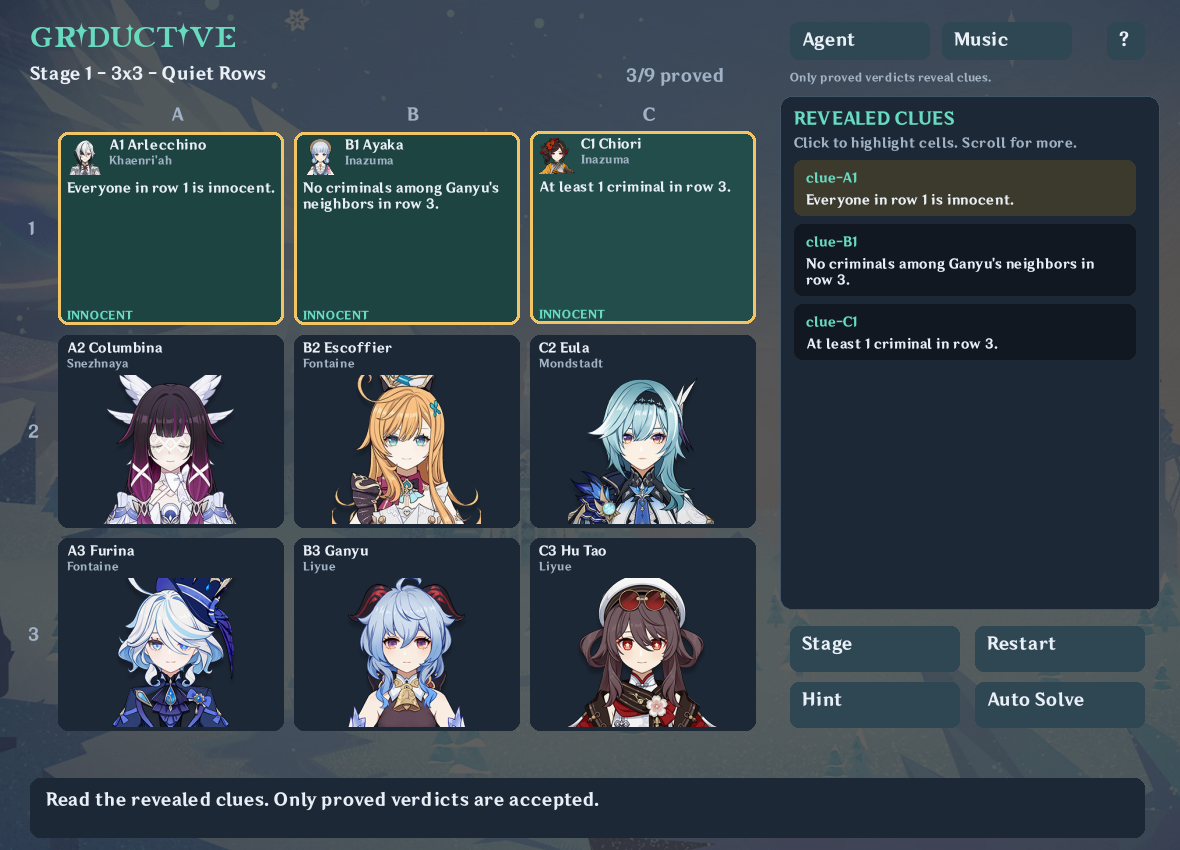
\includegraphics[width=0.75\textwidth]{figures/gameplay.png}
    \caption{Giao diện trò chơi Griductive với bàn cờ và bảng manh mối.}
    \label{fig:gameplay}
\end{figure}

Các tính năng chính gồm:
\begin{itemize}
    \item \textbf{Chọn trạng thái nhân vật:} nhấp vào thẻ để chọn \texttt{Innocent} hoặc \texttt{Criminal}. Có thể dùng WASD/phím mũi tên để di chuyển và Enter để mở, xác nhận lựa chọn.
    \item \textbf{Mở thẻ và phản hồi:} kết luận hợp lệ sẽ mở thẻ, thu nhỏ ảnh và hiện manh mối. Chương trình phân biệt lựa chọn chưa đủ căn cứ (\texttt{NOT\_PROVABLE}) và lựa chọn bị manh mối bác bỏ (\texttt{CONTRADICTED}); cả hai đều giữ nguyên bàn cờ.
    \item \textbf{Chọn màn và chơi lại:} \texttt{Stage} hiển thị số thứ tự, kích thước và tên màn, chẳng hạn \texttt{Stage 1 - 3x3 - Quiet Rows}. \texttt{Restart} khôi phục các thẻ mở ban đầu và xóa lịch sử phân tích.
    \item \textbf{Gợi ý và giải tự động:} \texttt{Hint} chọn một nhân vật có thể chứng minh tiếp theo; \texttt{Auto Solve} mở lần lượt các thẻ theo kết quả suy diễn. Người chơi có thể dừng bằng \texttt{Stop}.
    \item \textbf{Quan sát tác tử:} \texttt{Agent} mở bảng bên cạnh trò chơi; cửa sổ mở rộng và co giãn theo màn hình. \texttt{Analyze} phân tích mà không mở thẻ, còn \texttt{Next move} thực hiện một lượt suy diễn và mở thẻ nếu có kết luận bắt buộc.
    \item \textbf{Hỗ trợ trải nghiệm:} bảng manh mối có thanh cuộn, các nút và thẻ có hiệu ứng tương tác, nút dấu hỏi mở hướng dẫn. Menu \texttt{Music} chứa danh sách bản nhạc và nút bật/tắt âm nhạc.
\end{itemize}

Trong bảng Agent, \texttt{Previous call}/\texttt{Next call} cho phép xem lại bàn cờ sau hành động tương ứng. Chế độ lịch sử chỉ đọc, không thay đổi trạng thái trò chơi đang chạy; \texttt{Live} đưa người chơi trở về bàn cờ hiện tại. Bảng cũng hiển thị số biến chính/phụ, mệnh đề CNF, lượt gọi SAT, quyết định, lan truyền, quay lui, bước suy diễn và thời gian, tách theo lượt phân tích và tổng tích lũy. Bộ đếm chưa được cung cấp hiển thị \texttt{N/A}.

Hình~\ref{fig:agent-inspector} minh họa bảng Agent khi sử dụng tác tử CNF/DPLL và xem lại một lượt phân tích trước đó.

\begin{figure}[!htbp]
    \centering
    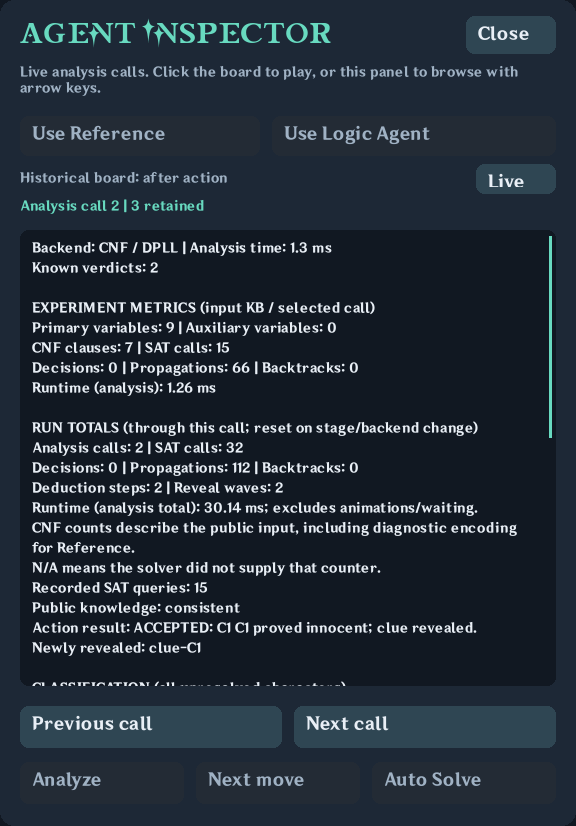
\includegraphics[width=0.8\textwidth]{figures/agent_inspector.png}
    \caption{Agent inspector hiển thị lịch sử phân tích và các chỉ số của tác tử CNF/DPLL.}
    \label{fig:agent-inspector}
\end{figure}

Ảnh nền, chân dung, phông chữ và âm nhạc được nạp từ \texttt{assets/}; nguồn được ghi tại \path{assets/ATTRIBUTION.md}~\cite{assetRecord}. Màu sắc, kích thước thẻ và thời gian hoạt ảnh được cấu hình trong \texttt{griductive/ui/config.py}.

\section{Tổ chức và tích hợp bộ phân tích}
\texttt{GameEngine} quản lý đáp án và các manh mối chưa mở. Bộ phân tích chỉ nhận \texttt{PublicState}, gồm thông tin nhân vật, trạng thái đã biết và manh mối công khai. Kết quả phân tích được engine sử dụng để chấp nhận hoặc từ chối lựa chọn; chỉ sau khi chấp nhận, trạng thái và manh mối mới được công khai.

Trò chơi mặc định dùng bộ phân tích tham chiếu bằng quay lui ngữ nghĩa. Repo hiện có bộ mã hóa CNF và bộ giải DPLL; người dùng chuyển giữa \texttt{Use Reference} và \texttt{Use Logic Agent} trong bảng Agent. Cả hai kết nối qua giao diện \texttt{analyze(PublicState) -> Analysis}. Nếu thành phần logic chưa khả dụng, tác tử có thể dùng bộ phân tích tham chiếu dự phòng và ghi rõ \texttt{Reference fallback}.

Tác vụ phân tích chạy trong luồng nền để giao diện tiếp tục xử lý sự kiện và hiển thị. Các ảnh chụp trạng thái công khai được lưu riêng cho chức năng xem lại; chỉ kết luận được engine chấp nhận mới mở thêm thẻ và được tính là bước suy diễn.
